  \chapter{Evaluation}\label{C:eval}

\section{Introduction}

Evaluation of this project is difficult as it is impossible to know exactly how many of the bugs that exist in the 42 compiler were found due to this project. It is hard, in practice, to prove that a complex software system is bug-free \cite{EWD:EWD249}. It is possible, but probably not likely, that the vast majority of bugs were found, and also possible, and probably more likely, that this project has barely scratched the surface of the bugs that could be found.

Overall this project has discovered a significant amount of bugs, with 32 previously unidentified bugs being found over the course of the project. The ratio of bugs found to tests written is also quite good, meaning that the effectiveness of each test written was relatively high.


\section{Evaluation Criteria}

It has been decided that this project will be evaluated based on two criteria, the quantity of bugs found, and the nature of the bugs found.

The first criterion was considered the more important as the aim of this project was to find bugs in the 42 compiler, therefore the higher the quantity of bugs found, the more successful the project has been. It was decided that the secondary evaluation criterion would be the categorisation of bugs. Before any bugs were found, eight separate categories that bugs were likely to fall into were decided upon (see Section \ref{cat} for these categories).

\subsection{Quantity of Bugs Found}

Quantity of bugs found is the first and most important criterion. Thirty-two bugs were found over the course of this project, and this is a good outcome for the project, as these bugs were unidentified bugs in the 42 compiler. It is difficult to place this number in context, but one way that has been done is to take the number of programs written over the course of this project, and divide this by the number of tests. This would provide the number of tests written for each bug found over the course of this project, and from this we can also determine the probability of any given test finding a bug. 

\begin{table}[h]
\centering
\begin{threeparttable}
 \caption{The categories and quantity of bugs found}
    \begin{tabular}{| l | c | c |}
    \hline
    \textbf{Category} & \textbf{Quantity} & \textbf{\% of Total Quantity} \\ \hline
    Syntax (too liberal) & 4 & 12.5 \\ \hline
    Syntax (too restrictive) & 4 & 12.5 \\ \hline
    Type system (too liberal) & 1 & 3.1 \\ \hline
    Type system (too restrictive) & 3 & 9.4  \\ \hline
    Metaprogramming (too liberal) & 0 & 0  \\ \hline
    Metaprogramming (too restrictive) & 1  & 3.1 \\ \hline
    Reduction & 6  & 18.8 \\ \hline
    Standard Library Bugs & 7 & 21.9 \\ \hline
    Miscellaneous &  6  & 18.8\\ \hline
    \textbf{Total quantity}	& \textbf{32}  & \textbf{100.1}  \tnote{1} \\ \hline
    \end{tabular}

  \begin{tablenotes}
    \item[1] Percentages do not add up to 100\% due to rounding.
  \end{tablenotes}

\end{threeparttable}


\end{table}

\subsection{Categorisation of Bugs Found \label{cat}}

Before any work beyond language familiarisation was carried out on the project, a set of eight different categories of bugs that were likely to be found was created by Dr. Servetto. This section will provide information on each category. The categorisation of the discovered bugs may not be completely accurate. A reason for this is the fact that some bugs are difficult to categorise, and do not fit nicely into a single category, or they may span over multiple categories. This means that the categorisation of the bugs is not a good tool on which to solely evaluate this project, and the quantity of bugs found therefore must also be taken into account.

\subsubsection{Syntax Bugs}

This category of consists of bugs that are considered to be related to the syntax of 42. This was most common category of bugs found over the course of this project, with eight bugs being found in this category, meaning that 25\% of bugs found were in this category. The large number of bugs in this category could be due to a few different reasons. Firstly, the syntax is extremely easy to test; every time a program is compiled and run the syntax is being tested in some way. Secondly, these bugs are generally easier to find than some other categories, such as the metaprogramming category, especially given the testing methodology employed in this project. 

This category is further split up into two different sub-categories: Syntax (too liberal) and Syntax (too restrictive). Too liberal syntax bugs would be bugs where the syntax is too free, and it allows a user to write 42 code that should not be allowed to compile, as it breaks some sort of syntax rule that should be enforced. Too restrictive syntax bugs are very similar to the too liberal syntax bugs except these bugs mean that a user can write code that meets the language specifications, but the compiler rejects it as syntactically incorrect. 

This category of bugs is generally due to their being a difference between the 42 specification and the implementation of the 42 compiler. This means that a bug falls into this category when during the compilation of the program, an error arises in code that the specification states should compile and run correctly.

\subsubsection{Type System Bugs}

This category consists of bugs that are considered to be related to the type system of 42. This category was the fifth most common category of bugs found over the course of this project, with four bugs being found in this category. With thirty-two bugs found overall, this means that 12.5\% of all bugs found in the course of this project fell into this category. These bugs were not particularly common due to the fact that the 42 type system is theoretically quite sound, and has a strong mathematical basis. 

This category, like the syntax category, can be split up into two sub-categories:  Type system (too liberal) and Type system (too restrictive). Too liberal type system bugs are bugs where the type system is too liberal, and code that is improperly typed is allowed to compile and be run. This code may still display the intended behaviour, depending on the specific bug, but it is still a bug as the compiler should have rejected the code as incorrect. Too restrictive type system bugs are where the type system is too restrictive and code that should have compiled and run correctly does not.

Type system bugs can present a major problem, especially when the type system is too liberal. In this case, code that should be rejected by the type system is accepted and this can lead to major problems when the program runs. When the type system is too restrictive a programmer may be forced to change the way their code works, even though according to the 42 specification it is correct.

The cause of this category of bugs is generally due to some kind of error in the implementation of the 42 compiler, or in rare cases, a difference between the 42 specification and implementation.

\subsubsection{Metaprogramming Bugs \label{meta}}

This category consists of bugs that are considered to be related to the metaprogramming features of 42. This category was the least common category of bugs found over the course of this project, with only one bug being found in this category. With thirty-two bugs found overall, this means that 3.1\% of all bugs found in the course of this project fell into this category. The lack of bugs found in this category probably stems from the lack of metaprogramming testing done for this project. Far fewer tests focused on this category of bugs when compared to the other categories of bugs such as syntax or type system bugs. This was primarily due to a personal lack of knowledge of metaprogamming beyond the basics. Research was done into metaprogramming but it was difficult to gain the knowledge required to thoroughly test the metaprogramming features whilst juggling the other demands of this project. It is known that metaprogramming bugs do exist in the project, as Dr. Servetto has found some examples during his own research.

\subsubsection{Reduction Bugs}

This category includes bugs that are related to the reduction of 42 programs. This category was the third most common category of bugs found over the course of this project, with six bugs being found in this category. This means that 18.8\% of bugs found over the course of this project fell into this category. These bugs were fairly common as program reduction plays a major part in the 42 compilation process, and therefore any program that was compiled and run over the course of this project could have potentially found a bug that fell into this category. 

Reduction bugs are when there is a problem in the conversion process of 42 code into Java bytecode or through an error with javac. These bugs therefore generally take the form of the outputted compiled code's behaviour differing from the expected behaviour of the 42 program that was compiled.

\subsubsection{Standard Library Bugs}

This category consists of bugs in the 42 standard library, Adam's Towel. This category was the second most common category with seven bugs, or 21.9\% of the total found falling into this category.

Adam's Towel provides practically all the basic functionality of 42, apart from base language features like classes. This means that using any language features such as the number or string classes will test the standard library, therefore it is not surprising that finding bugs in this category was common. The bugs in this category took on a wide range of guises due the expansiveness of the standard library.

\subsubsection{Miscellaneous Bugs}

This category of bugs includes all the bugs that did not fit into any of the other previously discussed categories. This category was one of the more common categories of bugs found over the course of this project, with six bugs being found in this category. This means that 18.8\% of bugs found over the course of this project fell into this category. A reason for this is that any bug that did not fit nicely and cleanly into any other category was placed in this one. 



\section{Testing Method}

Overall, use case testing proved to be the most effective testing method used during this project. Use case tests identified twenty-five bugs (78\% of the total bugs) out of thirty-five bugs. This was probably due to a combination of this testing method being used for the majority of the tests, and the flexibility of the testing method.

Error guessing was the second most effective method of testing, with seven bugs found with this method (22\% of the total bugs). More bugs were found with this method than expected, primarily because it was used for longer than was initially planned.

Orthogonal squares was the least effective method of testing with no bugs being identified with this method. This is partially because, due to the lack of effectiveness, the use of this method was discontinued.

\begin{figure}[h]
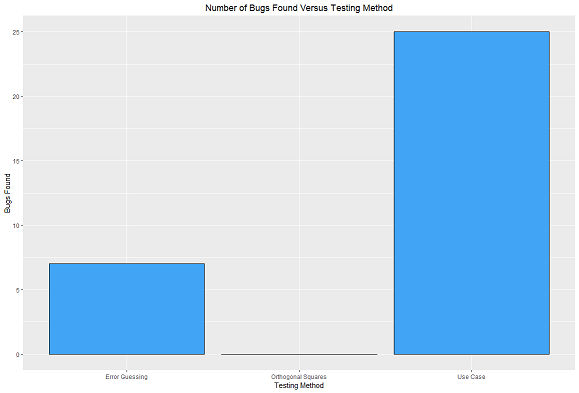
\includegraphics{bugsvmeth}
\caption{A bar graph showing how many bugs each testing method found \label{graph}}
\end{figure}


\section{Overall Evaluation}



\subsection{Quantity Calculations}

Over the course of this project many programs were written and 246 programs were kept, either by being turned into automated tests, or being saved as they were interesting in some way. This is not truly reflective of the number of programs written over the course of this project, because quite often, tests were very similar to previously written tests. This led to the belief that there was not much value in saving them. Only tests that found a bug, or were considered to be unique or interesting were saved. In hindsight, this was a flaw in the project design, as it made it harder to evaluate the overall success of the project. Keeping all the programs and therefore having an accurate number of the tests written would have been helpful for the evaluation.

 This means that any calculations made in regards to the probability of a bug being found per test are potentially flawed, but they still can have some value, especially if a estimation on the total number of programs written is made.

A conservative estimate of the total number of programs written over the course of this project would be around 2,500. This number could be much higher and this estimate is a lower bound that will be used for calculations in the next section. However many of these programs were only slightly different, such as a method parameter being slightly tweaked. There were not 2,500 wholly unique programs created.

\subsubsection{Probability of Finding a Bug}

A useful evaluation metric for this project is the effectiveness of the tests that were written. A good way of measuring the effectiveness of the tests written is calculating how many tests were required to find a single bug. 

If the number of tests written is taken as 246, we can divide this number by the number of bugs found (32), giving an equation of $ 246 / 32 $, which gives an answer of 7.69 tests written for each bug found. This is an low number of tests per bug found, and is an unrealistic representation of the effectiveness of the testing carried out over the course of this project. This is because, as mentioned previously, unfortunately not all the programs that were written were saved, and the number of programs written was not accurately recorded. With the previous estimate of written programs being around 2,500, we can do $ 2500 / 32 $, which gives an answer of 78.13 tests written for each bug found. This is a much more reasonable number of tests when compared to the previous answer of 7.69 tests written per bug found. It is still a low number of tests per bug found, especially when compared to more established languages where thousands of programs can be written without finding a single bug. The reciprocal of the number of tests written per bug found can be taken, and this will give the probability of any given test written over the course of this project finding a bug.

~\\
If we take the number of tests written as 246 we get
\[ \dfrac{1}{246 / 32} \]
\[ = 0.13 \]
Or a probability of $p = 0.13$ of any given test finding a bug.

~\\
If we take the number of tests written as 2,500 we get
\[ \dfrac{1}{2500 / 32} \]
\[ = 0.0128 \]
Or a probability of $p = 0.0128$ of any given test finding a bug.

~\\


\subsection{Bugs Found Over Time}

Over the course of this project, as time went on, the number of bugs found decreased (see Figure \ref{graph}). This could suggest that a significant portion of the bugs in the compiler have been found over the course of this project, as less were found as time went on. However this claim should be approached cautiously, as correlation does not imply causation, but a trend can be seen in terms of the number of bugs found over time. 
\begin{figure}[h]
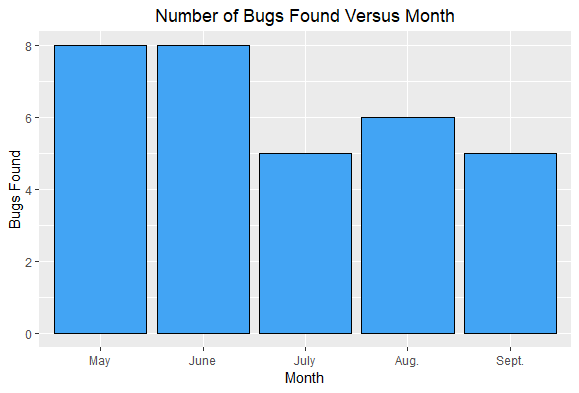
\includegraphics{bugsvsmonth}
\caption{A bar graph showing how many bugs were found per month \label{graph}}
\end{figure}
Alternate reasons for the decreasing number of bugs found could involve changes in the testing method used, or the number of tests written. Overall, this data shows that the number of bugs found over time decreased, but caution should be taken when drawing any conclusions from this data alone.


\section{Summary of Evaluation}

In order to gain an accurate and fair evaluation of this project, the two evaluation criteria previously mentioned, quantity of bugs, and categorisation of bugs, have been used in conjunction. The overall quantity of bugs found was thirty-two, which is a large number of bugs to find in a compiler, especially when considering the fact that they were previously unknown bugs. 

This number can be put in context by taking into account how many tests were written to identify these bugs over the course of this project. 246 programs were recorded as have being written, but not all programs were recorded, and at a conservative estimate, 2,500 tests were written of the course of this project. All evaluation conclusions based off 246 tests will be severely flawed and not accurately reflect the effectiveness of the testing carried out. Therefore the figure of 2,500 programs written will be used for evaluation purposes. Using this figure, 78.13 tests were written for each bug found. This is a very good ratio, and clearly shows that the testing carried out was effective.

The large number of syntax, reduction, and type system bugs found show that the testing carried over the course of this project was quite effective in some areas, but the lack of bugs found in other areas such as metaprogramming shows that there were weak points in the testing.

Overall, finding thirty-two bugs, and finding a bug every seventy-eight tests shows that the testing carried out for this project was effective and well targeted. Finding bugs was the main goal of this project, therefore it can be stated that this project was, on the whole, successful.
